%!TeX program = xelatex
\documentclass[12pt,hyperref,a4paper,UTF8]{ctexart}
\usepackage{HDUReport}
\usepackage{listings}
\usepackage{xcolor}
\usepackage{graphicx}
\usepackage{setspace}
\usepackage{float}
\setstretch{1.5} % 设置全局行距为1.5倍

\usepackage{enumitem} % 载入enumitem包以便自定义列表环境
\setlist[itemize]{itemsep=0pt, parsep=0pt} % 设置itemize环境的项目间距和段落间距

\setmainfont{Times New Roman} % 英文正文为Times New Roman

%封面页设置
{   
    %标题
    \title{ 
        \vspace{1cm}
        \heiti \Huge \textbf{电子信息虚拟仿真实验报告} \par
        \vspace{1cm} 
        \heiti \Large {\underline{实验3:PWM控制器设计}   } 
        \vspace{3cm}
    
    }

    \author{
        \vspace{0.5cm}
        \kaishu\Large 学院\ \dlmu[9cm]{卓越学院} \\ %学院
        \vspace{0.5cm}
        \kaishu\Large 学号\ \dlmu[9cm]{23040447} \\ %班级
        \vspace{0.5cm}
        \kaishu\Large 姓名\ \dlmu[9cm]{陈文轩} \qquad  \\ %学号
        \vspace{0.5cm}
        \kaishu\Large 专业\ \dlmu[9cm]{智能硬件与系统(电子信息工程)} \qquad \\ %姓名 
    }
        
    \date{\today} % 默认为今天的日期,可以注释掉不显示日期
}
%%------------------------document环境开始------------------------%%
\begin{document}

%%-----------------------封面--------------------%%
\cover
\thispagestyle{empty} % 首页不显示页码
%%------------------摘要-------------%%
%\newpage
%\begin{abstract}




%\end{abstract}

%\thispagestyle{empty} % 首页不显示页码

%%--------------------------目录页------------------------%%
\newpage
\tableofcontents
\thispagestyle{empty} % 目录不显示页码

%%------------------------正文页从这里开始-------------------%
\newpage
\setcounter{page}{1} % 让页码从正文开始编号

%%可选择这里也放一个标题
%\begin{center}
%    \title{ \Huge \textbf{{标题}}}
%\end{center}

\section{顶层电路设计(verilog)}


\begin{figure}[H]
    \centering
    \begin{minipage}{1\textwidth}
        \centering
        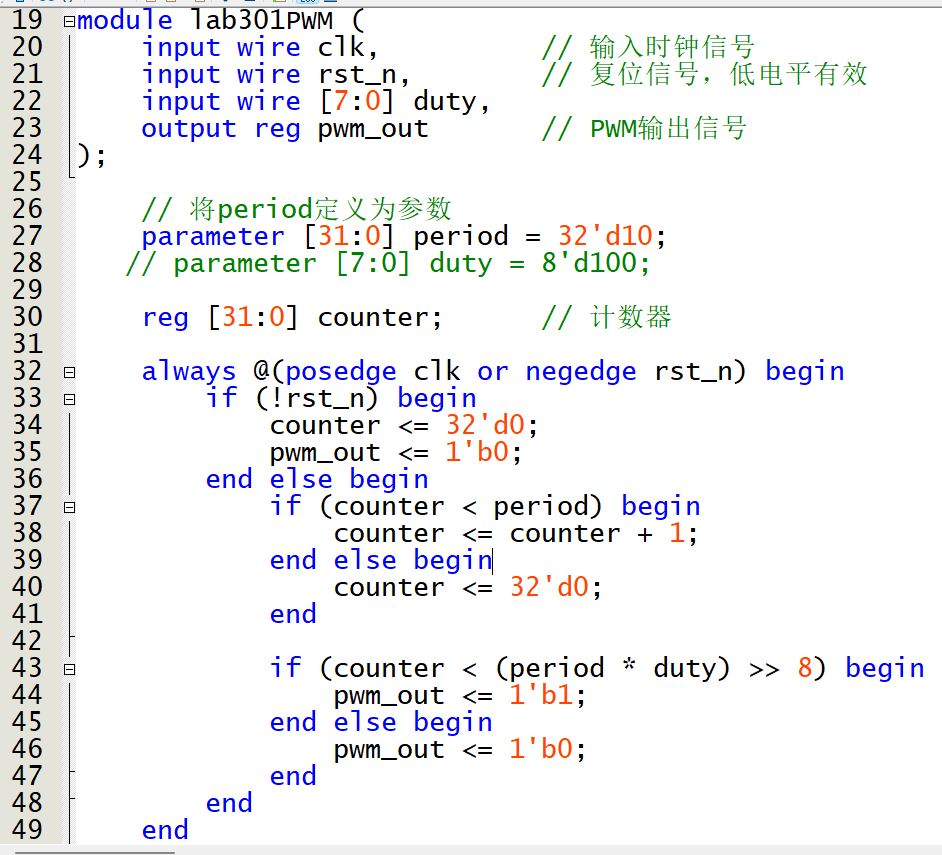
\includegraphics[width=1\textwidth]{figures/301.png}
        \caption{顶层电路设计(verilog)}
        \label{fig:system_block_diagram}
    \end{minipage}
\end{figure}

\section{仿真结果电路截图}

\begin{figure}[H]
    \centering
    \begin{minipage}{1\textwidth}
        \centering
        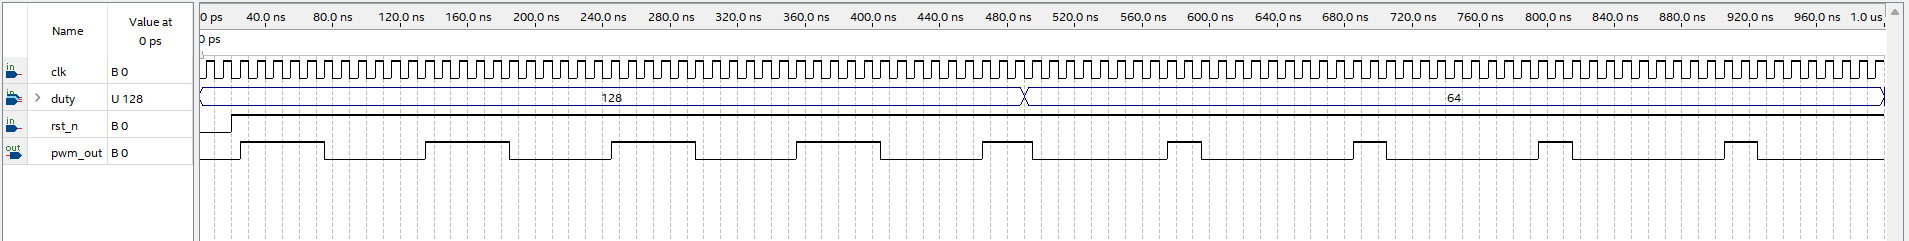
\includegraphics[width=1\textwidth]{figures/601.png}
        \caption{VWF仿真结果}
        \label{fig:system_block_diagram}
    \end{minipage}
\end{figure}

\section{远程平台操作截图}


\begin{figure}[H]
    \centering
    \begin{minipage}{0.8\textwidth}
        \centering
        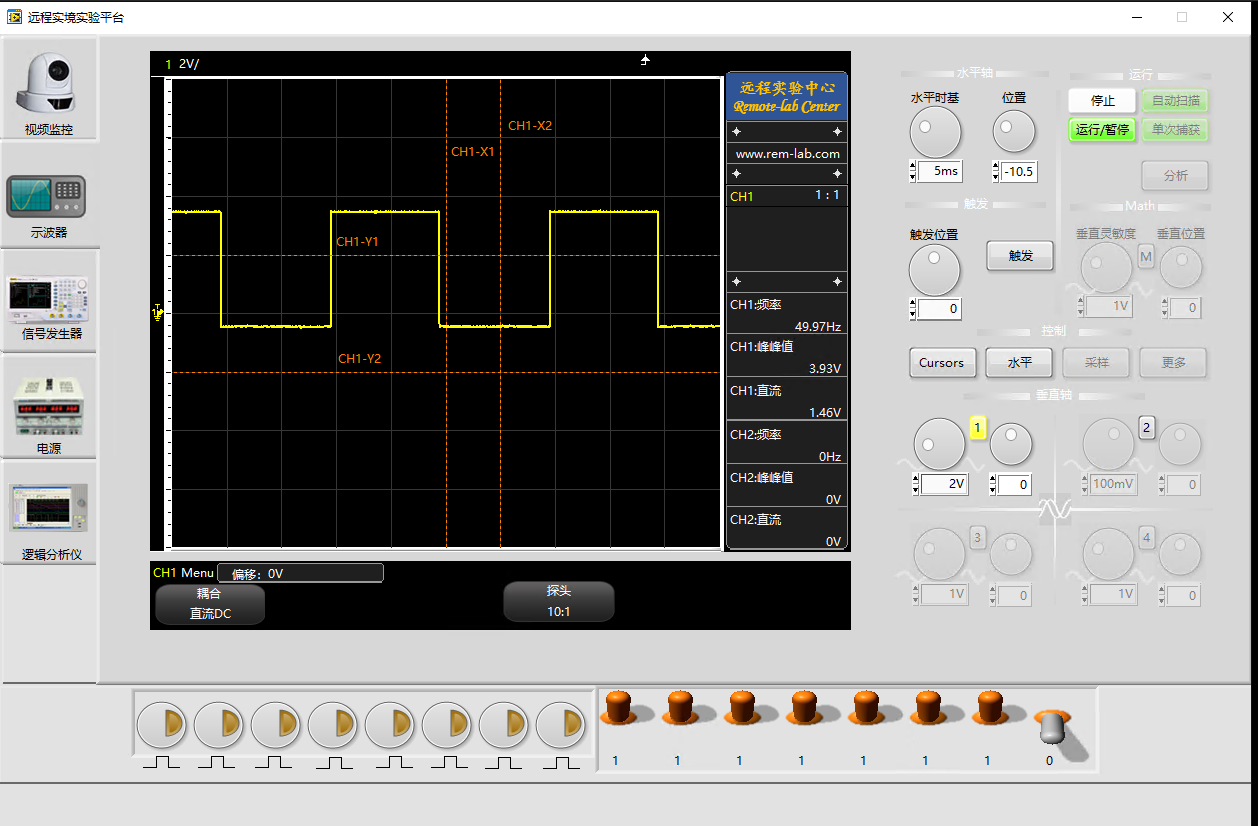
\includegraphics[width=0.8\textwidth]{figures/501.png}
        \caption{操作截图:50HZ方波}
        \label{fig:system_block_diagram}
    \end{minipage}
\end{figure}


\begin{figure}[H]
    \centering
    \begin{minipage}{0.8\textwidth}
        \centering
        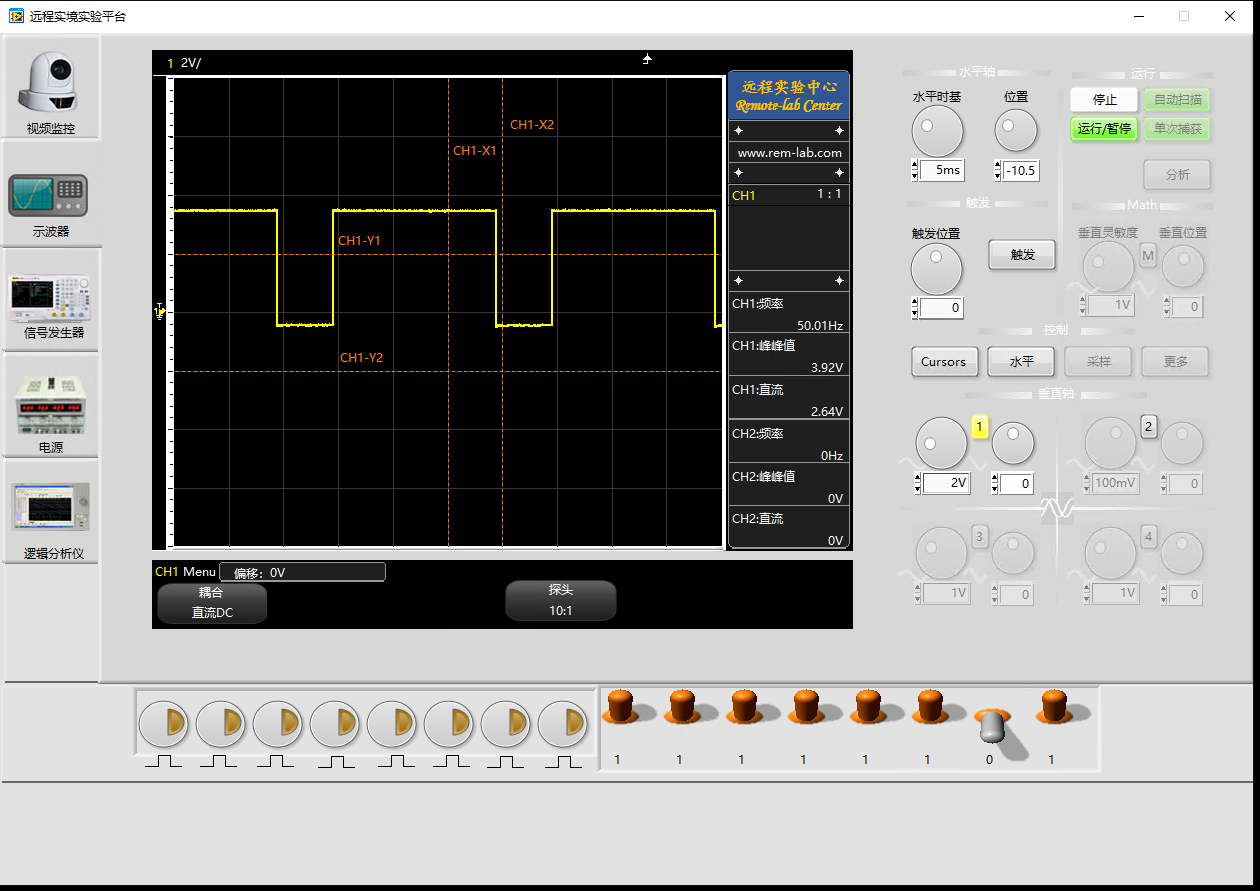
\includegraphics[width=0.8\textwidth]{figures/502.png}
        \caption{操作截图:50HZ矩形波,占空比8'b10111111/8'd256=0.746}
        \label{fig:system_block_diagram}
    \end{minipage}
\end{figure}
\begin{figure}[H]
    \centering
    \begin{minipage}{0.8\textwidth}
        \centering
        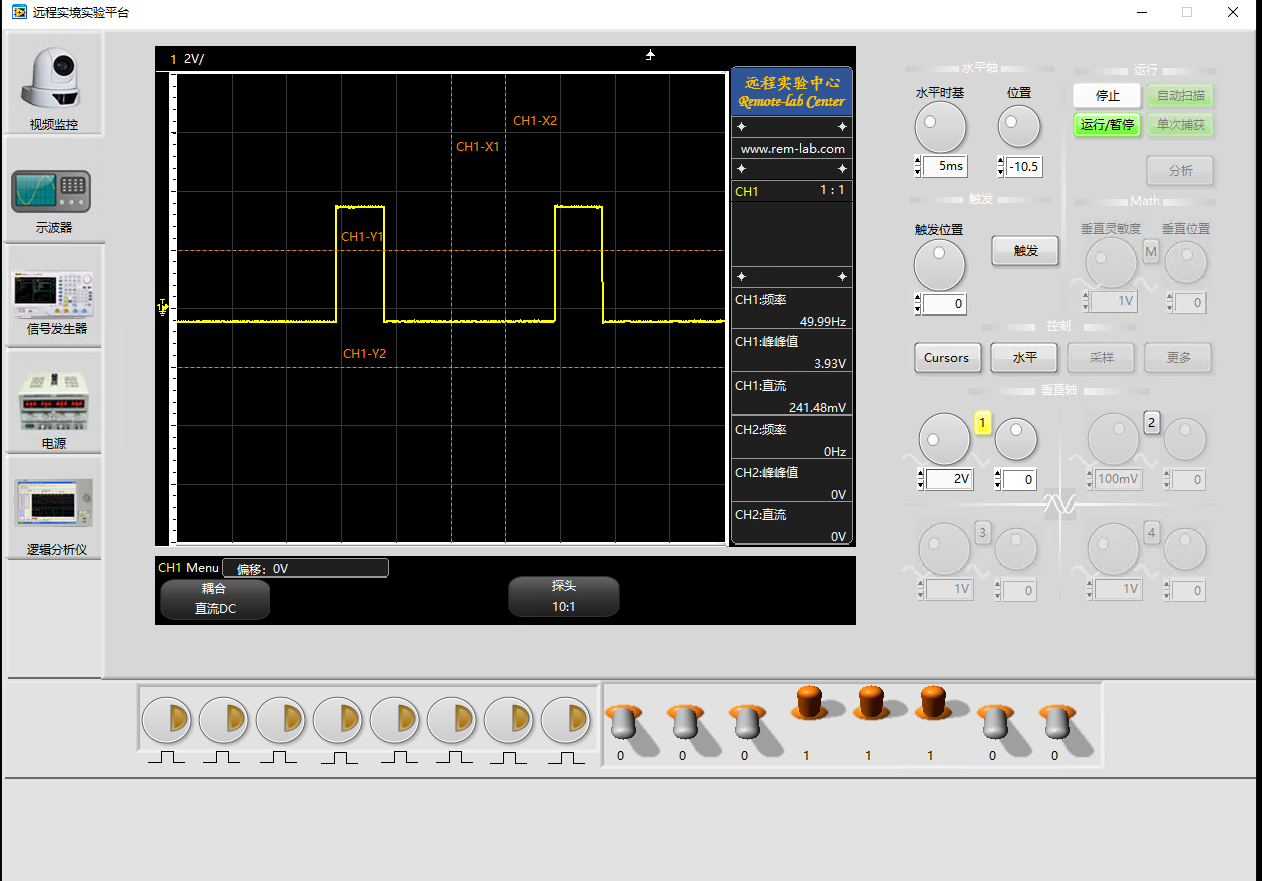
\includegraphics[width=0.8\textwidth]{figures/503.png}
        \caption{操作截图:50HZ矩形波,占空比8'b00111000/8'd256=0.219}
        \label{fig:system_block_diagram}
    \end{minipage}
\end{figure}


\section{实验设计过程简要介绍}

\subsection{实验概述}
本实验设计了一个基于Verilog的PWM(脉宽调制)信号生成模块,能够通过调整占空比和周期参数生成不同频率和占空比的PWM信号。实验内容包括模块设计、仿真验证以及硬件实现。

\subsection{模块设计}
\subsubsection{顶层模块 \texttt{lab301PWM}}
\begin{lstlisting}[language=Verilog]
module lab301PWM (
    input wire clk,          // 输入时钟信号
    input wire rst_n,        // 复位信号,低电平有效
    input wire [7:0] duty,   // 占空比控制信号
    output reg pwm_out       // PWM输出信号
);
\end{lstlisting}

\subsubsection{主要功能组件}
\begin{enumerate}
    \item \textbf{计数器模块}
    \begin{itemize}
        \item 计数器 \texttt{counter} 用于记录当前时钟周期。
        \item 当计数器值达到设定的周期 \texttt{period} 时复位为0。
    \end{itemize}
    
    \item \textbf{占空比控制逻辑}
    \begin{itemize}
        \item 根据占空比信号 \texttt{duty} 和周期 \texttt{period} 计算高电平持续时间。
        \item 当计数器值小于 \texttt{(period * duty) >> 8} 时,输出高电平,否则输出低电平。
    \end{itemize}
\end{enumerate}

\subsection{实验内容}
\subsubsection{PWM信号生成模块设计与仿真验证}

PWM信号生成模块通过以下步骤实现:
\begin{enumerate}
    \item 计数器 \texttt{counter} 在每个时钟周期递增,直到达到设定的周期 \texttt{period},然后复位为0。
    \item 根据占空比信号 \texttt{duty} 计算高电平持续时间:
    \[
    \text{High\_Time} = \frac{\text{period} \times \text{duty}}{256}
    \]
    \item 当计数器值小于高电平持续时间时,输出 \texttt{pwm\_out} 为高电平,否则为低电平。
\end{enumerate}

仿真测试应覆盖以下场景:
\begin{itemize}
    \item 不同占空比测试:如0\%、50\%、100\%。
    \item 不同周期测试:如周期为10、100、1000。
    \item 边界值测试:如占空比为0和255。
\end{itemize}

\subsubsection{硬件实现与测试}
将设计的PWM模块下载到FPGA开发板,通过示波器观察输出信号波形,验证以下功能:
\begin{enumerate}
    \item PWM信号的频率与设定的周期 \texttt{period} 一致。
    \item PWM信号的占空比与输入的 \texttt{duty} 信号一致。
\end{enumerate}

\subsection{关键模块说明}
\subsubsection{计数器模块}
计数器用于生成周期性信号,其实现如下:
\begin{lstlisting}[language=Verilog]
if (counter < period) begin
    counter <= counter + 1;
end else begin
    counter <= 32'd0;
end
\end{lstlisting}

\subsubsection{占空比控制逻辑}
占空比控制逻辑根据计数器值和占空比信号生成PWM输出:
\begin{lstlisting}[language=Verilog]
if (counter < (period * duty) >> 8) begin
    pwm_out <= 1'b1;
end else begin
    pwm_out <= 1'b0;
end
\end{lstlisting}

\subsection{实验总结}
本实验成功实现了:
\begin{enumerate}
    \item 基于Verilog的PWM信号生成模块设计。
    \item PWM信号的占空比和频率可调。
    \item 仿真验证和硬件测试均表明模块功能正确。
\end{enumerate}

通过本实验,掌握了PWM信号的基本原理及其在数字电路中的实现方法,为后续复杂数字系统设计奠定了基础。







\end{document}

